\subsection{Deconvolution of the array response}

As can be seen in fig. \ref{fig:4mic1srcInd}, even in ideal conditions, the localization results from SRP-PHAT contain many peaks of varying heights. This is due to summing the cross-correlation responses of a non-linear array (Eq. \ref{eq:srpSumInd}). If the array was linear, the localization circles from each pair would all overlap completely. In case of a tetrahedral array, the localization circles from the possible microphone pairs are not co-planar. This is because all the edges of a tetrahedron point in the different directions. The obvious problem here is in multi-source detection. If multiple sources are playing at different levels, how do we determine if a detected peak is a real source or a pseudo-source from another higher level source? The methods to do so form the basis of deconvolution methods for SRP-PHAT.

\subsection{Deconvolution history}
Coming Soon!
\newpage
\subsubsection{Product-SRP-PHAT}
A simple deconvolution approach could be to penalize sources which are only detected by a subset of the microphone pair combinations. This could be done by taking a product and not a sum in Eq. \ref{eq:srpSumInd}.
\begin{equation}
    S_{SRP}(\theta,\phi)=\prod\limits_{i=1}^{M-1}{R_{x_0,x_i}[f_{0,i}(\theta,\phi)]}
     \label{eq:srpProdInd}
\end{equation}
This way, if a peak is caused by a single localization circle, the cross-correlation values from other microphone pairs would be close to zero, and thus would scale the false peak down. The localization results from this are given in fig. \ref{fig:4mic1srcNoisyProd}.
\begin{figure}[H]
    \centering
    \begin{subfigure}[b]{0.96\textwidth}
    \centering
    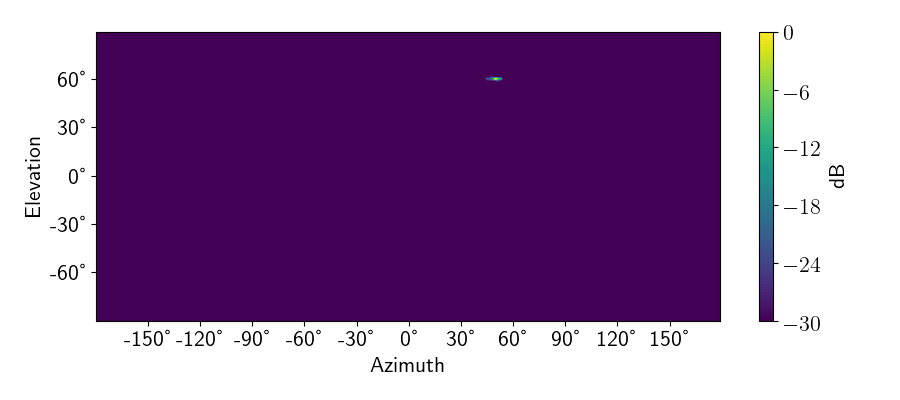
\includegraphics[width=0.8\textwidth]{Figures/Ind4mic1srcProd20.png}
\end{subfigure}
\vskip \baselineskip
\begin{subfigure}[b]{0.96\textwidth}
    \centering
    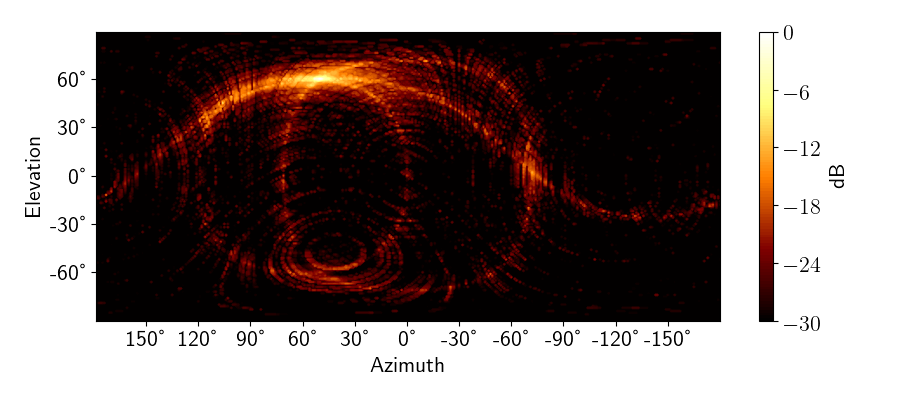
\includegraphics[width=0.8\textwidth]{Figures/Ind4mic1srcProd0.png}
\end{subfigure}
\vskip \baselineskip
\begin{subfigure}[b]{0.96\textwidth}
    \centering
    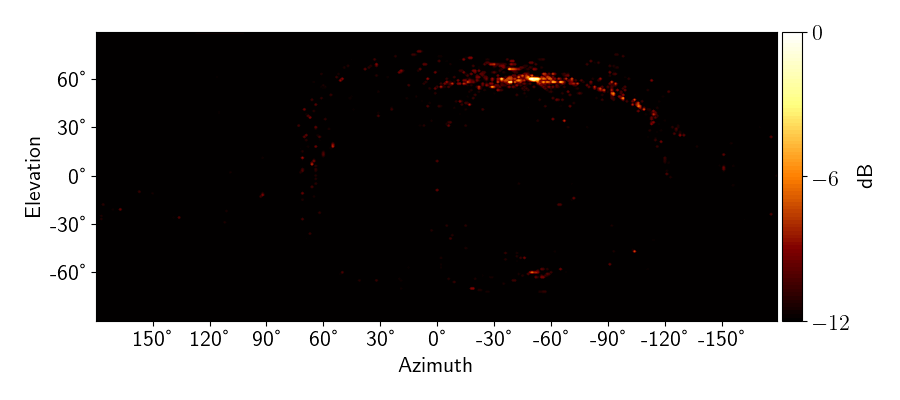
\includegraphics[width=0.8\textwidth]{Figures/Ind4mic1srcProdNeg10.png}
\end{subfigure}
\caption{Figures depict from top-to-bottom product-SRP-PHAT localization results  with SNR = 20dB, SNR = 0dB, SNR = -10dB}
\label{fig:4mic1srcNoisyProd}
\end{figure}
\newpage
The drawback of using product-SRP-PHAT is that the sound level difference between the different sound sources is lost. In normal SRP-PHAT, the array magnitude response at a particular azimuth and elevation is averaged over all microphone pair combinations. Then the level difference between 2 sources is maintained. In product-SRP-PHAT this would not be the case. However if it is assumed that a particular source will have similar magnitude response for all microphone pairs (which is not a strong assumption in far-field), then taking source power $P_{SRP}={S_{SRP}}^{1/M}$, the level difference can be maintained.  Fig. \ref{fig:4mic2srcNoisyCompare} depicts the results of product-SRP-PHAT after level correction.
\begin{figure}[H]
    \centering
    \begin{subfigure}[b]{0.96\textwidth}
    \centering
    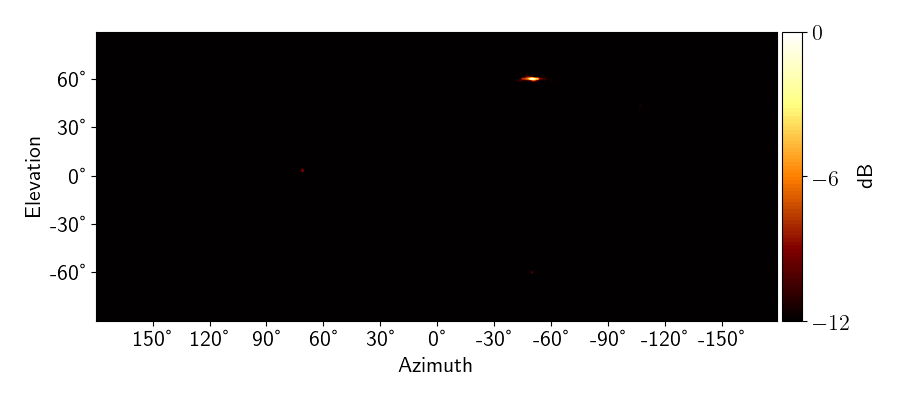
\includegraphics[width=0.8\textwidth]{Figures/Ind4mic1srcProd20Corr.png}
\end{subfigure}
\vskip \baselineskip
\begin{subfigure}[b]{0.96\textwidth}
    \centering
    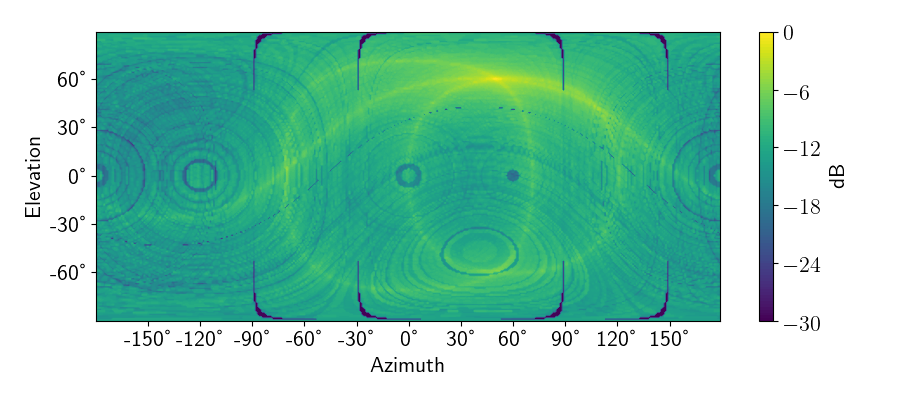
\includegraphics[width=0.8\textwidth]{Figures/Ind4mic1srcProd0Corr.png}
\end{subfigure}
\vskip \baselineskip
\begin{subfigure}[b]{0.96\textwidth}
    \centering
    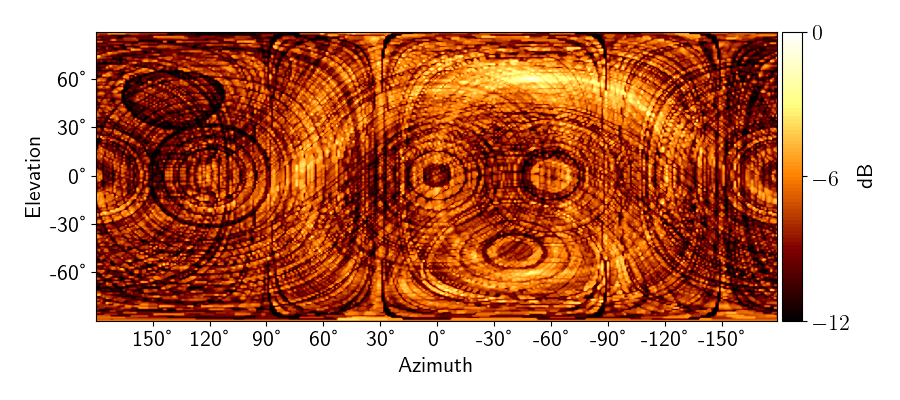
\includegraphics[width=0.8\textwidth]{Figures//Ind4mic1srcProdNeg10Corr.png}
\end{subfigure}
\caption{Figures depict from top-to-bottom level corrected product-SRP-PHAT localization results with SNR = 20dB, SNR = 0dB, SNR = -10dB}
\label{fig:4mic2srcNoisyCompare}
\end{figure}
\subsubsection{Minimum power SRP-PHAT}
Another deconvolution approach can be to use the far-field assumption again, to assume that the power received from a single source to all microphone pairs is the same. In that case, if, the minimum power between the microphone pair is assumed to be the true power (instead of summing), peaks which are detected only by a subset of microphone arrays would disappear automatically and the deconvolution problem can be solved directly. Fig. \ref{fig:4mic1srcNoisyMinPow} shows the results. Even in adverse conditions of 0 dB, the algorithm is fairly able to detect the source at $(50\degree, 60\degree)$, without any subsidiary peaks due to the localization cones. 
\begin{figure}[H]
    \centering
    \begin{subfigure}[b]{0.96\textwidth}
    \centering
    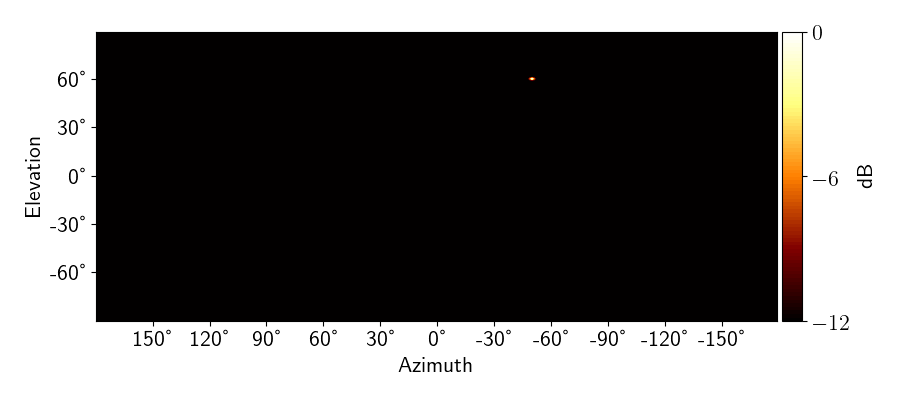
\includegraphics[width=0.8\textwidth]{Figures/Ind4mic1srcMin20.png}
\end{subfigure}
\vskip \baselineskip
\begin{subfigure}[b]{0.96\textwidth}
    \centering
    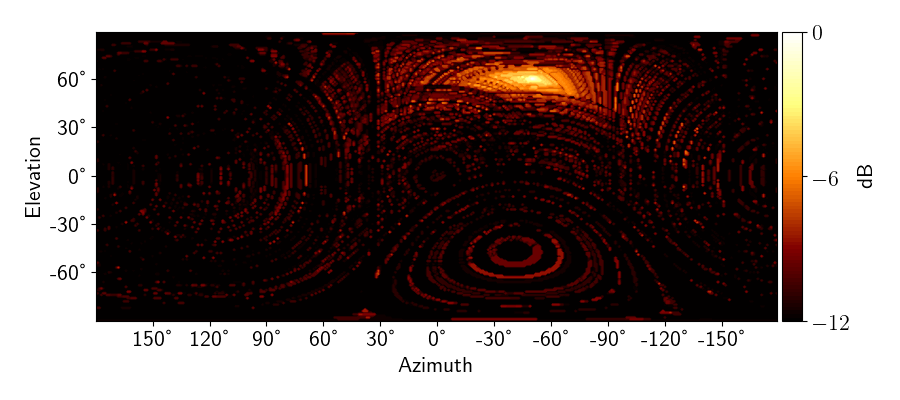
\includegraphics[width=0.8\textwidth]{Figures/Ind4mic1srcMin0.png}
\end{subfigure}
\vskip \baselineskip
\begin{subfigure}[b]{0.96\textwidth}
    \centering
    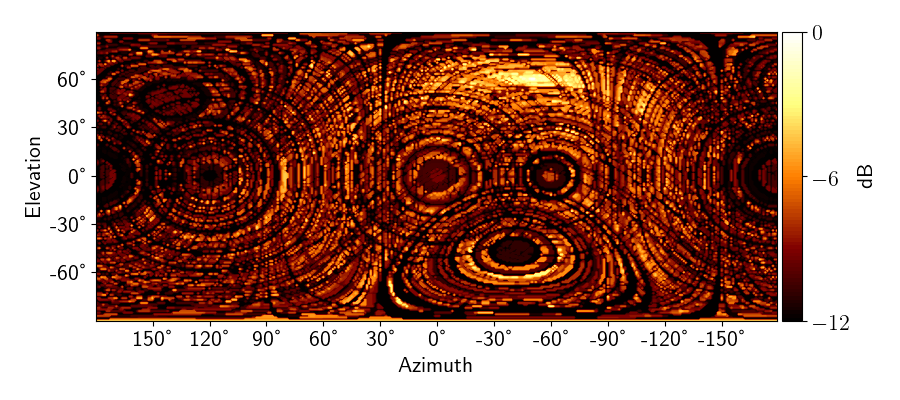
\includegraphics[width=0.8\textwidth]{Figures/Ind4mic1srcMinNeg10.png}
\end{subfigure}
\caption{Figures depict from top-to-bottom minimum power SRP-PHAT localization results with SNR = 20dB, SNR = 0dB, SNR = -10dB}
\label{fig:4mic1srcNoisyMinPow}
\end{figure}
Minimum power SRP-PHAT is same in principle to finding the intersection of multiple hyperboloids, since this method only returns sound sources detected by all independent microphone pairs. The drawback of both product-SRP-PHAT and Minimum power SRP-PHAT is that in case of localizing point sources, even a minor error in temperature or wind recordings has the potential of not detecting the sound source completely. However, since outdoor sound sources are usually large, the cones from microphone pairs are not sharp circular lines, rather, they are broad depending on the sound source size. An error in weather conditions would then cause these fatty circles to `smudge' together. Since minimum power picks the lowest powered circle for each point searched, this has the potential to underestimate the sound source, both in size and magnitude.

\subsection{Other Deconvolution methods}
CLEAN is an algorithm proposed by Jan Högbom in 1974 \cite{1974A&AS...15..417H} to perform the deconvolution of images in radio astronomy. Högbom observed the sky images being polluted by what he described as the "dirty beam". This "dirty beam" is the distortion introduced in the system output when the input is subject to a point source. It relates to the point spread function (PSF) in optic or the array response in our case. The CLEAN algorithm removes the side lobes of the beamformer when the PSF is known in advance throught simulation or measurement. CLEAN-SC is an extension of the CLEAN algorithm but does not rely on knowing the PSF in advance, it uses the coherence between the sidelobes and the main beam to identify the PSF and retrieve the level of the sources. Usually efficient deconvolution is performed in the frequency domain when the PSF is shift-invariant but in our case the PSF change for every scanned position as the array response is different therefore it can become challenging to perform the deconvolution on a real time system. The CLEAN and CLEAN-SC algorithm and some notation will be introduced as well as the algorithm issues. Methods to overcome those issues are also discussed.

\subsubsection{CLEAN deconvolution of the beamformed maps}

The energy map obtained with the SRP-PHAT algorithm is composed of N sound sources of complex amplitude $\hat{A_{N}}$ convoluted with the array response $p(t)$ and some noise n(t). This "image" I(t) can be expressed as in equation \ref{eq:imageclean}
\begin{equation}
    I(t)=\sum\limits_{n=1}^{N}{A_{n}p(t-t_{n})+n(t)}
    \label{eq:imageclean}
\end{equation}

In real situation it might be difficult to retrieve the sources information in this noisy map. A naive and straightforward solution consist in subtracting the array response of the strongest peak and so on until there is no prominent peak left on the map. By subtracting the array response (PSF), a residual image $I_{m}$ is created.

\begin{equation}
    I_{m}(t)=I(t)-\hat{A}_{m}p(t-\hat{t}_{m})
\end{equation}

This idea is among the line of the CLEAN algorithm where usually a fraction of the PSF is deconvoluted from the map. However this method has several drawbacks such as assuming the main peak to be a source and not an addition of interferences created by other sources. Also it assumes the number of sources to be known in advance. To overcome this problem and retrieve the real sources among interferences, a PSF correlation algorithm has been described in \cite{freedman1995techniques}. The PSF Correlation algorithm define the minimal target mass criterion as follow:

\subsubsection{The PSF correlation algorithm}

    \begin{equation}
        M_{m}=\int_{-\infty}^{\infty}|{(I_{m}(t))}|^2
    \end{equation}
    
    \begin{equation}
        \begin{split}
        M_{m} & =\int_{-\infty}^{\infty}\{{(I(t)-\hat{A}_{m}p(t-\hat{t}_{m})}\}\{{(I(t)-\hat{A}_{m}p(t-\hat{t}_{m})}\}^*dt \\
              & = M + |{\hat{A}_{m}}|^2M_{p}-2Re[{\hat{A}_{m}}{R^*_{pl}(\hat{t}_{m})}]\\
              & = M + |{\hat{A}_{m}}|^2M_{p}-2|{\hat{A}_{m}}||{R_{pl}(\hat{t}_{m})}|cos(\hat{\alpha}_{m}-\phi(\hat{t}_{m})
        \end{split}
    \end{equation}

$M_{p}$ is the mass of the point spread function and $R_{pl}(\hat{t_{m}})=\int_{-\infty}^{\infty}{p^{*}(t-\hat(t_{m})I(i)dt}$ is the cross-correlation function between the image and the PSF.
The intuition of the PSF correlation algorithm is that there exists an optimal position $\hat{t}$ which minimize this criteria. This optimal target position to cancel can then be inputed in the CLEAN Algorithm itself.\\

\subsubsection{CLEAN-SC deconvolution of the beamformed maps}

The CLEAN method is attractive in simulation as the cones intersect in one point but as explained earlier it will never happen in practice, there will never be clean cone intersections in the beamformed results due to microphone error position, speed of source shift or wind effect. It is therefore challenging to know what PSF to substract from the map since there is no clean peak in the map. CLEAN-SC is an addition to the CLEAN methods but no assumption about the PSF is made and the PSF is retrieved using the coherence information between the main lobes and the side lobes. The algorithm also retrieves the sources amplitudes, it is interesting to note that the computation time of the CLEAN-SC is usually twice the one to compute the beamformed map, as stated earlier no real time implementation is considered but it is nevertheless interesting to note. CLEAN-SC \cite{sijtsma2007clean} has been published in 2007 by Pieter Sijtsma and the algorithm basics will be explained in this section. Let's first define the Cross Spectrum Matrix (CSM) $\hat{C}$ given by
\begin{equation}
\hat{C}=
    \begin{bmatrix} 
      C_{11} & C_{12} & \cdots & C_{1m_{0}}\\
      \vdots &  C_{22} &       &  \vdots\\
      \vdots &         & \ddots &  \vdots\\
      C_{m_{0}1} &     &       &  C_{m_{0}m_{0}}\\
    \end{bmatrix}  
\end{equation}
where $C_{mm'}$ is the cross spectrum between microphone m  and m'. It is computed by taking the FFT of the pressure recording $p^{*}_{mk}(t)$ and $p_{m'k}(t)$ averaged over K data blocks. $w_{s}$ is a weight filter like Hamming window.
\begin{equation}
    C_{mm'}=\frac{2}{Kw_{s}T}\sum\limits_{k=0}^{K}[P^{*}_{mk}(f,T)P_{m'k}(f,T)]
\end{equation}

Usually a trimmed CSM is used in order to only get the information of independent pairs of microphones, ie all the possible (m,n) combinations of microphones forming the subset S, with m and n the microphones indices. The trimmed CSM  ${\xoverline{C}_{mn}}$ is defined in equation \ref{eq:trimmedcsm}

\begin{equation}
     \xoverline{C} = 
      \begin{cases} 
       C_{mn} & \text{for } (m,n) \in S \\
       0      & \text{for } (m,n) \notin  S
      \end{cases}
    \label{eq:trimmedcsm}
\end{equation}

Let's now define the degraded CSM  $D^{i}$ when source components are removed and the CSM induced by peak source steering vector , $G^{i}$. The indice i is due to the process being iterative as sources are removed from the map. The source cross powers $B_{jk}$ is defined by the equation \ref{eq:crosspow} 

\begin{equation}
    B_{jk}=w_{j}^{*}\xoverline{C}w_{k}
    \label{eq:crosspow}
\end{equation}

with w, the weight vector defined from the steering vector as in equation \ref{eq:weightcsm}

\begin{equation}
    w=g/\sum\limits_{m,n\in S}(|{(g_{m})}|^2|{(g_{n})}|^2)^{1/2}
    \label{eq:weightcsm}
\end{equation}

The CLEAN-SC algorithm demands the source cross-powers of any scan point to be determined entirely by $G^{i}$.

\begin{equation}
    w_{j}^{*}{\xoverline{D}}^{i-1}w^{i}_{k}=w_{j}^{*}\xoverline{G}^{i}w^{i}_{k} 
\end{equation}

This equation has several solution but we can assume the $G^{i}$ to due to a single coherent source component $h^{(i)}$. 

\begin{equation}
    G^{i}=P_{max}^{(i-1)}h^{i}h^{*(i)}
\end{equation}


